%% FIXME do I need to change out [. . .] for \ldots?

%% FIXME - Be sure I got all of the blockquotes right

\newcommand\hallfigure[4]{
	\begin{figure}
		\centering
		\includegraphics[width=3in]{#1}
		\caption{{#2}---{#3}}
		\label{#4}
	\end{figure}
}

\chapter[Truth, Beauty, and the Reflection of God]{Truth, Beauty, and the Reflection of God: John Ruskin’s \textit{Seven Lamps of Architecture} and \textit{The Stones of Venice} as Palimpsests for Contemporary Architecture}

\author{Mark R. Hall, Ph.D.}

\begin{abstract}
Architecture is invariably shaped by both its creator and the
landscape from which it emerges.  These elements are inextricably
intertwined to produce a structure that is aesthetically pleasing,
philosophically erudite, and fully functional.  Nowhere is this more
clearly established than with John Ruskin, a noteworthy Victorian art
and social critic.  His \textit{Seven Lamps of Architecture} and
\textit{The Stones of Venice} serve as palimpsests for contemporary
architecture.  A link to the past is forged based on foundational
moral, ethical, philosophical, and religious principles that are
reflected in the structures themselves.  For Ruskin, when first
principles are applied, aesthetic integrity is maintained, truth and
beauty are manifested, and the reflection of God is contained in the
building itself.  The architecture may also point beyond itself to
something else, complementing it, expanding it, or transforming it
(such as in Gothic architecture).  Applying these Ruskinian laws and
virtues to today’s architecture provides a framework that grounds the
discipline in meaningful theological and philosophical underpinnings
from which inspiration and creativity may emerge.  Contemporary
examples include Daniel Libeskind’s Jewish Museum Berlin that opened in
2001 and Peter Eisenman’s Holocaust Memorial built in Berlin in 2004. 
Daniel Libeskind is also an architect for the One World Trade Center
scheduled to be opened in 2014.  The approach taken by these men to
design these structures demonstrate their philosophy that architecture
should arise out of history and landscape.  Therefore, the principles
of Ruskin function as a palimpsest for the inspiration, creativity, and
designs of architects like Eisenman and Libeskind, as they seek to
recapture and maintain the past through structures that promote their
own interpretation of memory and beauty, and also reflect truth, power,
and life.
\end{abstract}

\section{The Seven Lamps of Architecture}

John Ruskin in \textit{The Seven Lamps of Architecture} (1845) defines
architecture as ``the art which so disposes and adorns the edifices
raised by man [. . .] that the sight of them may contribute to his
mental health, power, and pleasure''\citep[][pg. 8]{ruskin1920}.  He asserts that
good architecture must exhibit seven lamps that represent spirits or
laws: sacrifice, truth, power, beauty, life, memory, and obedience. 
Ruskin sees these as the framework for architectural creation and
design.  He believes that good and beautiful architecture must conform
to these laws, and the observer should see that ``there is room for the
marking of his [man’s] relations with the mightiest, as well as the
fairest, works of God; and that those works themselves have been
permitted, by their [the architects’] Master and his [man’s], to
receive an added glory from their association with earnest efforts of
human thought''\citep[][pg. 73]{ruskin1920}.  According to Ruskin, architecture that reflects
these seven lamps will draw the builder and the observer toward an
experience with the Master Builder, God.  

In \textit{The Seven Lamps of Architecture}, Ruskin explains the
meaning of the seven lamps.  The illustration below (Figure \ref{fig:lamps_conceptual}) shows the
connections that exist among these seven laws.\citep[][pg. 402]{baljon1997}

\begin{enumerate}
\item 
Sacrifice – Architecture is an offering to God demonstrating men’s “love
and obedience and surrender of themselves and theirs to His will”\citep[][pg. 16]{ruskin1920}
as evidenced by the building of beautiful, ornate churches.  
\item 
Truth – Builders must use honest and true materials—crafted by human
hands, not machines—respecting them and rejecting false ones. 
\item 
Power – The construction of buildings must focus on mass, quantity of
shadow, breadth, sense of surface, size, weight, and shadow; the
efforts of the builders through their imagination should point toward
the sublimity and majesty of nature. 
\item 
Beauty – Architecture should point individuals toward God and reflect
the design and decoration found in nature.  
\item 
Life – Buildings should bear the mark of human hands, celebrating the
irregularity in design to show that the ornamentation is not mechanical
and demonstrating the joy of the builders as they construct with
freedom. 
\item 
Memory – Architecture should respect the social, historical, and
cultural character of its milieu, distinguishing between essential and
inessential forms.  
\item 
Obedience – Originality must recognize and be restrained by obedience to
tradition, especially connecting with the English architecture that has
preceded it. 
\end{enumerate}

\begin{figure}[H]
	\centering
	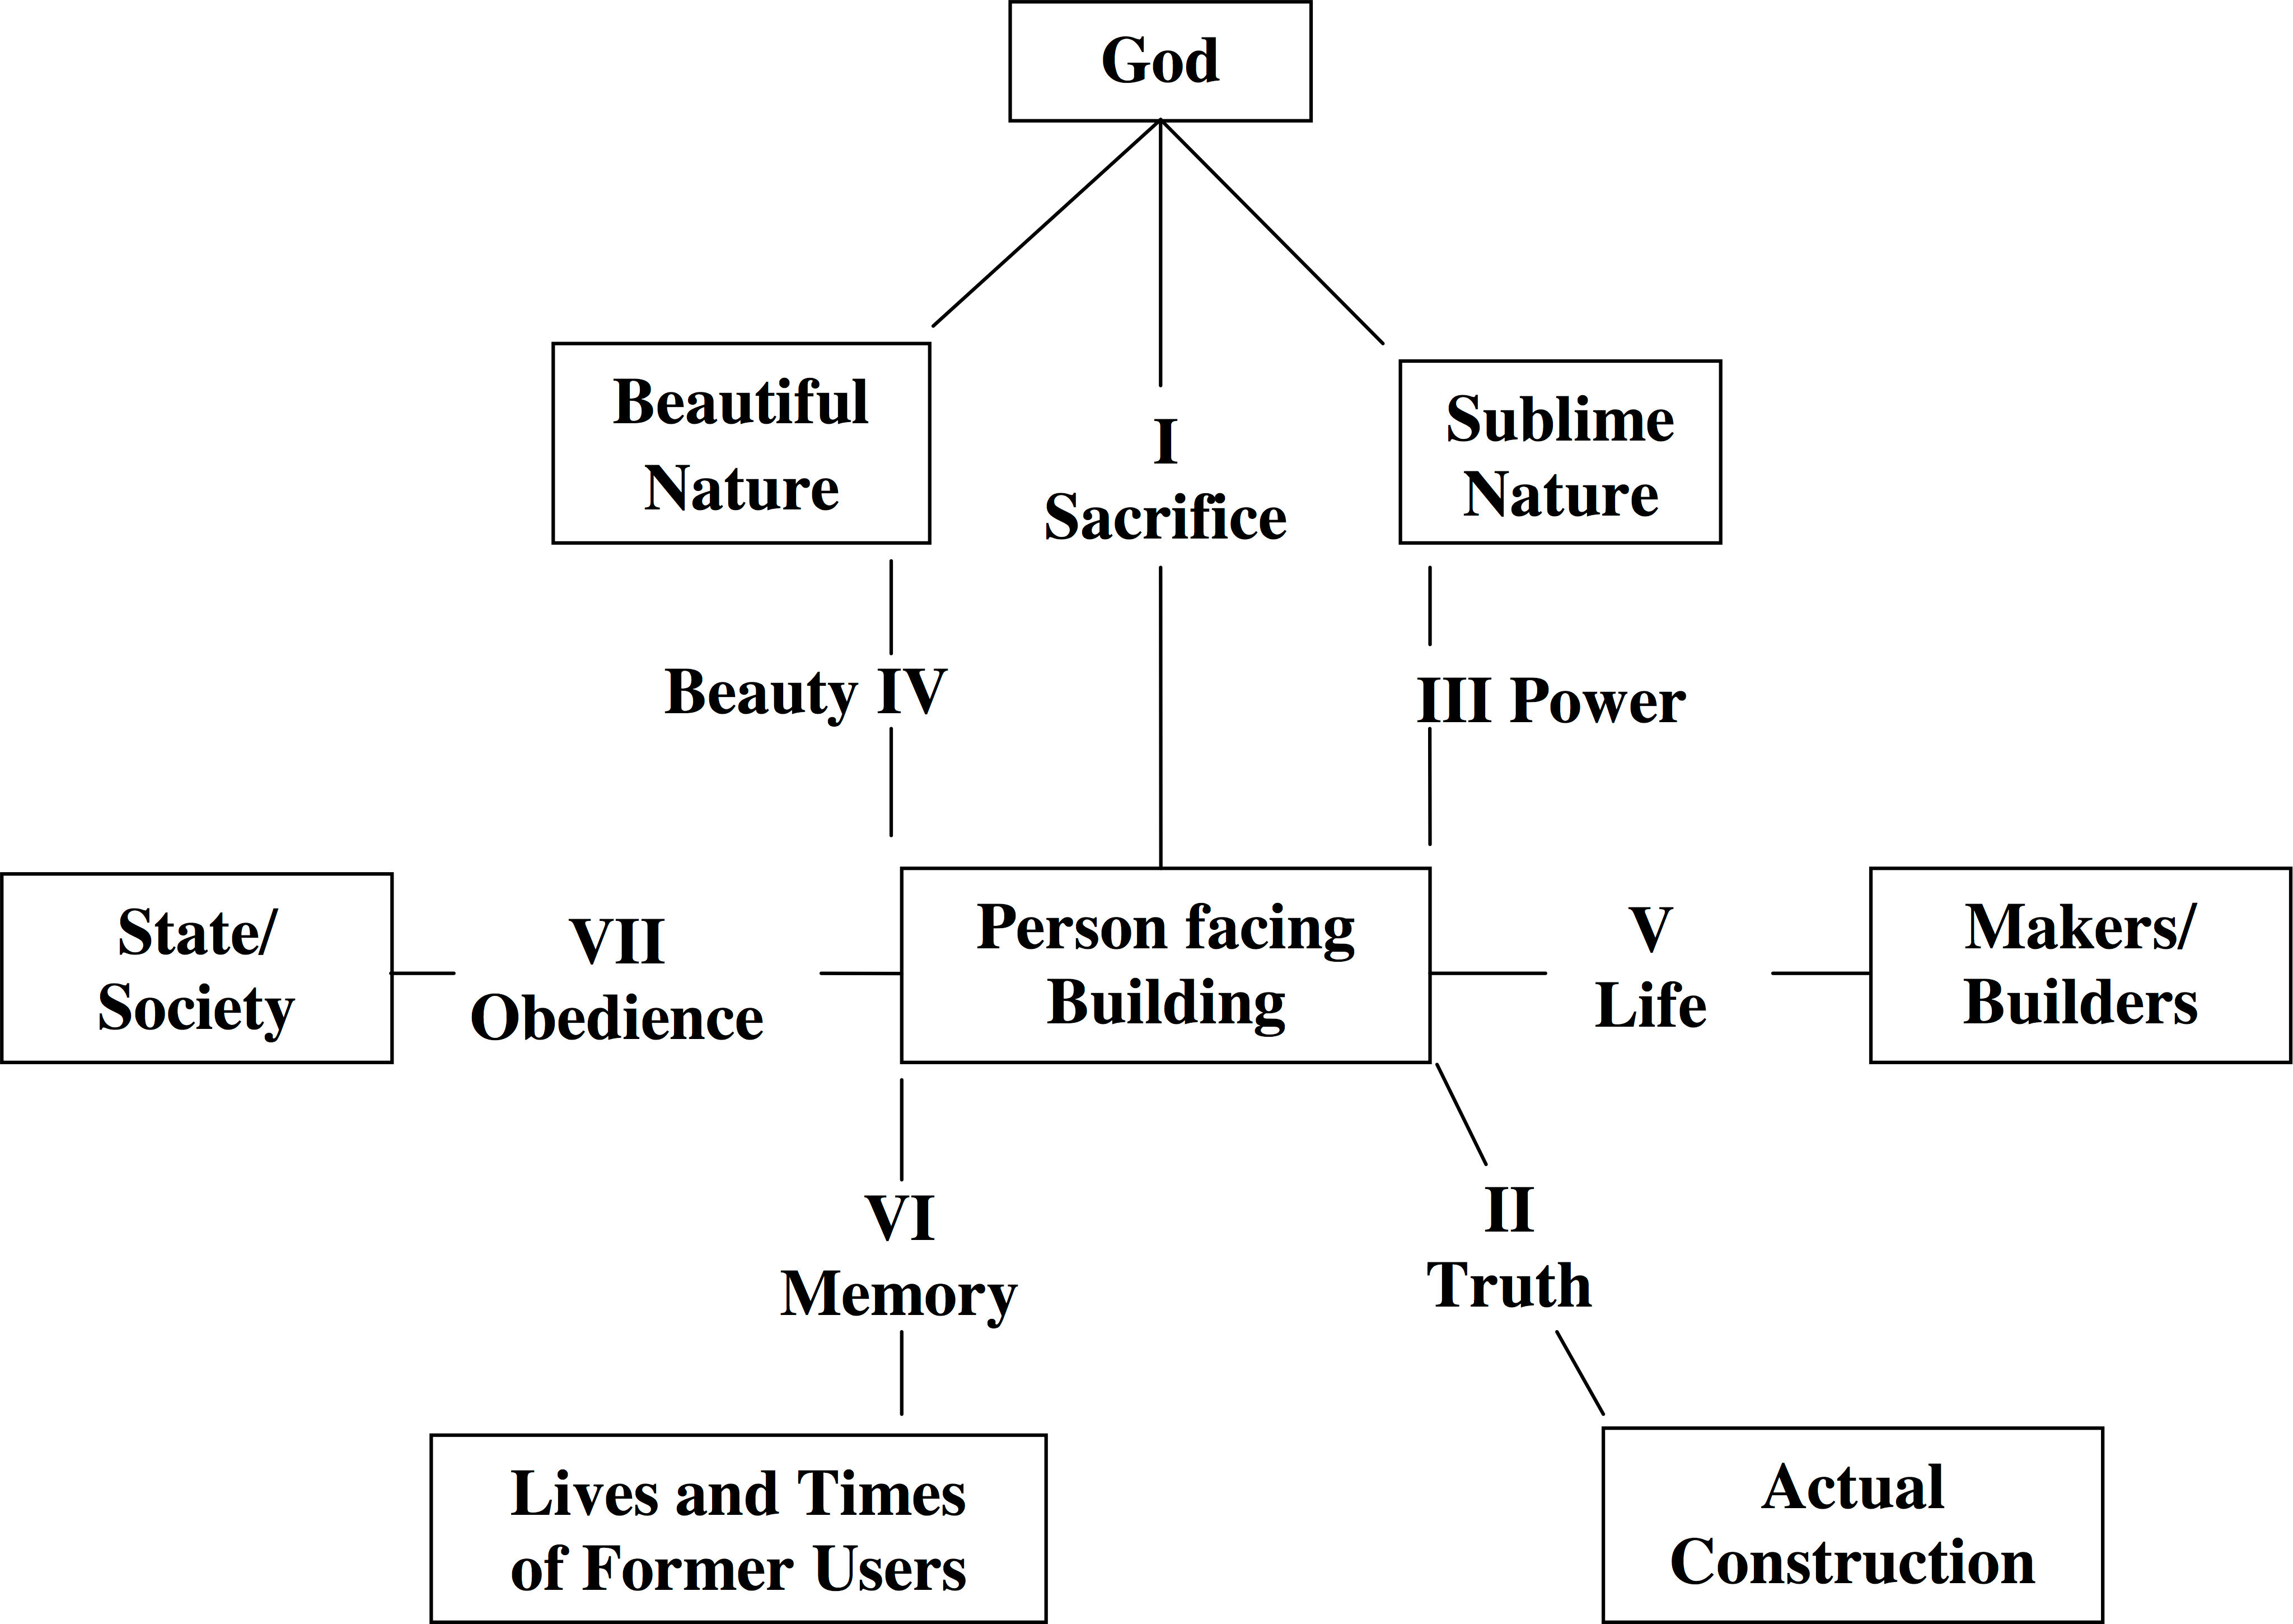
\includegraphics[width=5in]{HallChart.png}
	\caption{Conceptual Scheme of \textit{The Seven Lamps of Architecture}}
	\label{fig:lamps_conceptual}
\end{figure}

Ruskin ties beauty to human beings and their experience with nature in
\textit{The Seven Lamps of Architecture}.  In one diary entry dated
April 19, 1846, Ruskin describes a day in Champagnole, France and then
comments on how nature affected him: 

\begin{quote}
I felt it more than usual, but it struck me suddenly how utterly
different the impression of such a scene would be, if it were in a
strange land and in one without history.  How dear to the feeling is
the pine of Switzerland compared to that of Canada!  I have allowed too
little weight to these deep sympathies, for I think, if that pine
forest had been among the Alleghanys, or if the stream had been
Niagara, I should only have looked at them with intense melancholy and
desire for home.\citep[][pg. 325]{ruskin1956}
\end{quote}

This observation of creation enables Ruskin to embrace the theory of
associationism, especially its connections to history, which influences
his aesthetic appreciation.  George Landow points out that Ruskin’s
emphasis on beauty seems to emerge out of these historical associations
that assist his criticism of contemporary architecture.  Ruskin finds the homes and
public buildings of his England constructed without style, without
regard to permanence and without meaning for the men who inhabit them. 
Since he wishes to correct these deficiencies, he places great emphasis
upon historical associations, whose presence, he says, will insure both
that an edifice influence the life of the inhabitant and that it be
solidly constructed — this latter because if a building is to endure
long enough for historical associations to accrue, then it must be well
made. 

Thus, Ruskin’s establishment of memory as one of his seven laws—with its
focus on the social, historical, and cultural milieu—becomes essential
to his philosophy of architecture. 

\section{Ruskin and \textit{The Stones of Venice}}

%% FIXME - figure references
\hallfigure{HallImage1.jpg}{St. Mark's Cathedral, by John W. Bunney}{Public Domain}{fig:stmarks}

In \textit{The Stones of Venice,} Ruskin’s vivid description of St.
Mark’s Cathedral (Figure \ref{fig:stmarks}), a most magnificent structure in Venice---“the
most precious building in Europe standing yet in the eyes of men and
the sunshine of heaven”\citep{nyt1880}---and his detailed sketches of the
same (Figures \ref{fig:stmarkssouth}, \ref{fig:stmarksarchivolt}, \ref{fig:stmarksbasket}, \ref{fig:stmarksfacade}, \ref{fig:stmarksnorthwest}, and \ref{fig:stmarkssketch}) demonstrate the ability of the author to pen with
passion and eloquent style, and the artist to draw with precision and
color, the beauty of its architecture: 

\hallfigure{HallImage2.jpg}{The South Side of St. Mark's from the Loggia of the Ducal Palace, Venice, \~1851, by John Ruskin}{Public Domain}{fig:stmarkssouth}

\hallfigure{HallImage3.jpg}{Archivolt in St. Mark's, 1853, by John Ruskin}{Public Domain}{fig:stmarksarchivolt}

\hallfigure{HallImage4.jpg}{Basket and Lily Capital, St. Mark's Basilica, Venice, 1849--1852, by John Ruskin}{Public Domain}{fig:stmarksbasket}

\begin{quote}
A multitude of pillars and white domes, clustered into a long low
pyramid of coloured light; a treasure-heap, it seems, partly of gold,
and partly of opal and mother-of-pearl, hollowed beneath into five
great vaulted porches, ceiled with fair mosaic, and beset with
sculpture of alabaster, clear as amber and delicate as ivory —sculpture
fantastic and involved, of palm leaves and lilies, and grapes and
pomegranates, and birds clinging and fluttering among the branches, all
twined together into an endless network of buds and plumes; and, in the
midst of it, the solemn form of angels, sceptred, and robed to the
feet, and leaning to each other across the gates, their figures
indistinct among the gleaming of the golden ground through the leaves
beside them, interrupted and dim, like the morning light as it faded
back among the branches of Eden, when first its gates were
angel-guarded long ago.  And round the walls of the porches there are
set pillars of variegated stones, jasper and porphyry, and deep-green
serpentine spotted with flakes of snow, and marbles, that half refuse
and half yield to the sunshine, Cleopatra-like, ``their
bluest veins to kiss''---the shadow, as it steals back from
them, revealing line after line of azure undulation, as a receding tide
leaves the waved sand; their capitals rich with interwoven tracery,
rooted knots of herbage, and drifting leaves of acanthus and vine, and
mystical signs, all beginning and ending in the Cross; and above them,
in the broad archivolts, a continuous chain of language and of life—
angels, and the signs of heaven and the labours of men, each in its
appointed season upon the earth; and above these another range of
glittering pinnacles, mixed with white arches edged with scarlet
flowers,—a confusion of delight, amidst which the breasts of the Greek
horses are seen blazing in their breadth of golden strength, and the
St. Mark's Lion, lifted on a blue field covered with
stars, until at last, as if in ecstacy, the crests of the arches break
into a marble foam, and toss themselves far into the blue sky in
flashes and wreaths of sculptured spray, as if the breakers on the Lido
shore had been frost-bound before they fell, and the sea-nymphs had
inlaid them with coral and amethyst.  \citep[][vol. 2, ch. 4, sec. 14]{ruskin1885}
\end{quote}

\hallfigure{HallImage5.jpg}{Northwest Angle of the Fa\c{c}ade, St. Mark's Church, 1851, by John Ruskin}{Public Domain}{fig:stmarksfacade}

These words and drawings reflect the magnificence that resonates in the
actual architecture, authenticating the lamp of beauty, for Ruskin
clearly believes that architecture should reflect the design found in
nature and point towards the ultimate Master Builder.  

With a philosophy based on aesthetics, place, and history, Ruskin
appeals to a moral architecture, encouraging builders to reject the
techniques discovered in the Renaissance and developed in the
Industrial Revolution and to embrace a time when the best buildings
were constructed—the medieval Gothic cathedrals of England and Venice. 
In his later book, \textit{The Stones of Venice }(1851--1853), Ruskin
describes the elements of the Gothic that became foundational for the
kind of architecture he proposes, and he provides many examples to
illustrate.  He points out the three virtues of a building: (1) “That
it act well,” (2) “That it speak well,” and (3) “That it look well” \citep[][vol. 1, ch. 2, sec. 1]{ruskin1885}.  
In \textit{The Crown of Wild Olive}, Ruskin
explains the purpose of his writing: 

\hallfigure{HallImage6.jpg}{North West Porch, St. Mark's, Venice, 1877, by John Ruskin}{Public Domain}{fig:stmarksnorthwest}

\begin{quote}
The book I called ``The Seven Lamps'' was to show that certain right
states of temper and moral feeling were the magic powers by which all
good architecture, without exception, had been produced. 
``The Stones of Venice'' had, from beginning to end, no
other aim than to show that the Gothic architecture of Venice had
arisen out of, and indicated in all its features, a state of pure
national faith, and of domestic virtue; and that its Renaissance
architecture had arisen out of, and in all its features indicated, a
state of concealed national infidelity, and of  domestic corruption. 
\citep[][pg. 53]{ruskin1866}
\end{quote}

For Ruskin, moral feeling, states of temperament, and architecture
cannot be separated.  He sees the ``moral elements of Gothic'' as
follows: (1) savageness, (2) changefulness, (3) naturalism, (4)
grotesqueness, (5) rigidity, and (6) redundance, when “belonging to the
building,” and (1) savageness or rudeness, (2) love of change, (3) love
of nature, (4) disturbed imagination, (5) obstinancy, and (6)
generosity, when “belonging to the builder” \citep[][pg. 155]{ruskin1885}
.  Thus, Ruskin was not arguing for a new style of architecture. 
He was lamenting the plainness and the soullessness of the architecture
designed and built since the Gothic cathedrals of the medieval period. 
He “found certain
styles (e.g. Baroque) unacceptable because they exploited illusions,
and therefore were not `truthful'”\citep[][pg. 669]{curl2006}.
Therefore, according to Ruskin, in order for architecture
to be sincerely honest and truly beautiful, it must be connected to
nature, rooted in right history, and constructed by human hands.  

\section{Review of Ruskin's Reputation}

\hallfigure{HallImage7.jpg}{Part of St. Mark's, Venice, Sketch After Rain, 1846, by John Ruskin}{Public Domain}{fig:stmarkssketch}

The appeal of Ruskin’s philosophy of architecture was paramount during
the Victorian period.  Professor Robert Kerr, a contemporary of the art
critic, had previously espoused the same ideas as Ruskin, but he had
left them behind after working twenty years in the field.  He
encouraged experienced architects to deter younger apprentices from the
idealistic and romanticized views of Ruskin, for Kerr viewed the
architect as “a servant of the public for the efficient design of
buildings, precisely like the engineer.”  When he presented a lecture
entitled ``Architectural Criticism'' at the
Royal Institute of British Architects, he severely criticized Ruskin
saying that “Mr. Ruskin{\textquotesingle}s thoughts soar high enough in
the poetry of visionary art, because poetry is his business, but they
cannot stoop down to the plain prosaic details of the structuresque,
because building is not his business” \citep[][pg. 259--260]{collins1998}.  In an
October 1849 review of \textit{The Seven Lamps of Architecture
}published in the \textit{Journal of Design}, Matthew Digby Wyatt
admired “the excellent spirit” that was present in “this thoughtful,
eloquent book.”  However, he quickly points out that Ruskin “either
puts his back against  [. . .] further development, or would attempt to
bring back the world of art to what its course of actions was four
centuries ago!”\citep[][pgs. 121, 438]{mallgrave2009}

Ruskin does not hesitate to move from art critic to social critic,
demonstrating how the architecture itself can become a commentary on
the denigration, deterioration, and degradation of society.  Even as he
praises the majesty of St. Mark{\textquotesingle}s in \textit{The
Stones of Venice}, he also notes the ironic contrast that takes place
in its shadows as the masses ignore its beauty and the poor grovel in
their poverty.  

\begin{quote}
And what effect has this splendor on those who pass beneath it?  You may
walk from sunrise to sunset, to and fro, before the gateway of St.
Mark’s, and you will not see an eye lifted to it, nor a countenance
brightened by it.  Priest and layman, soldier and civilian, rich and
poor, pass by it alike regardlessly.  Up to the very recesses of the
porches, the meanest tradesmen of the city push their counters; nay,
the foundations of its pillars are themselves the seats—not “of them
that sell doves” for sacrifice, but of the vendors of toys and
caricatures.  Round the whole square in front of the church there is
almost a continuous line of cafés, where the idle Venetians of the
middle classes lounge, and read empty journals; in its centre the
Austrian bands play during the time of vespers, their martial music
jarring with the organ~notes,—the march drowning the miserere, and the
sullen crowd thickening round them,—a crowd, which, if it had its will,
would stiletto every soldier that pipes to it.  And in the recesses of
the porches, all day long, knots of men of the lowest classes,
unemployed and listless, lie basking in the sun like lizards; and
unregarded children,—every heavy glance of their young eyes full of
desperation and stony depravity, and their throats hoarse with
cursing,—gamble, and fight, and snarl, and sleep, hour after hour,
clashing their bruised centesimi upon the marble ledges of the church
porch.  And the images of Christ and His angels look down upon it
continually.\citep[][vol. 2, ch. 4, sec. 15]{ruskin1885}
\end{quote}

Ruskin observes that society and architecture are invariably connected.

John Matteson makes this observation concerning Ruskin the social
critic: ``The architecture was sublime; the human activity
around it was an obscene mockery.  What good was the building if it
could not transform the debauched children who cast lots on its very
steps?  After \textit{The Stones of Venice}, it was no longer enough
for Ruskin to criticize art.  It was hierarchies of human beings, not
structures of wood and stone, that begged most loudly for his
attention''\citep[][pg. 302]{matteson2002}.

\section{Ruskin's Relevance to Contemporary Architecture}

\hallfigure{HallImage8.jpg}{Crystal Palace, Sydenham, by Achille-Louis Martinet}{Public Domain}{fig:crystalpalace}

Clearly then Ruskin spoke to the Victorian period, but the question
inescapably arises, Can the aesthetic and moral philosophies of a
Victorian art and social critic be applicable to design and
construction today?  Is Ruskin relevant to contemporary architecture? 

\hallfigure{HallImage9.jpg}{Queen Victoria Opening the 1862 Exhibition (inside view of Crystal Palace), by Joseph Nash}{Public Domain}{fig:qvopening}

John Matteson discusses this very question.  Citing the building of the
Crystal Palace (Figures \ref{fig:crystalpalace} and \ref{fig:qvopening}), 
whose ``prefabricated components heralded a
revolution,'' which was occurring at the same time as the publication of
Ruskin{\textquotesingle}s \textit{Stones of Venice}, Matteson asserts
that ``Ruskin’s ideas were already destined for quaintness in the
1850s'' \citep[][pg. 300]{matteson2002}.  He points out some of the difficulties of
applying Ruskin{\textquotesingle}s first principles to contemporary
architecture: 

\hallfigure{HallImage10.jpg}{Cathedral of St. John the Divine, Wide Angle View}{Copyright \textcopyright 2011 Kirpaks and licensed for reuse under the Create Commons License Attribution-ShareAlike}{fig:stjohnwide}

\begin{quote}
Since Ruskin’s time, populations have grown and economic systems have
expanded with once unimaginable speed.  Construction in our time has to
be fast.  It must be efficient.  It must avoid unnecessary expense.  If
Ruskin foresaw the further mechanization of physical labor, he was at
least spared the sadness of seeing how far that mechanization would
eventually extend.  Ruskin also did not anticipate that the alienation
that he saw as poisoning the life of the worker might someday encompass
not only the process of construction, but also those of conception and
design.  He could never have imagined on-line catalogs of design
components or the idea that an architect might one day resolve
decisions of ornamentation, not with painstaking manual drawing or
model-building, but with the click of a mouse.  Neither could he have
expected that modern buildings would often be commissioned and
designed, not by individuals at all, but by impersonal organizations. 
It would have been strange, indeed, for Ruskin to discover the myriad
ways in which architecture could divorce itself from the simple human
acts of drawing and carving.\citep[][pg. 300]{matteson2002}
\end{quote}

Yet Matteson does not completely reject Ruskin’s writings about Gothic
architecture, citing the construction of St. John the Divine in
Manhattan (Figures \ref{fig:stjohnwide} and \ref{fig:stjohnwestern}) as an exemplar of Ruskinian ideals.  In 1972,
after no construction had occurred on the building for thirty years,
the dean of St. John the Divine proclaimed that it was time to once
again begin work and that “the stonework [would] be done by our own
unemployed and underemployed neighbors.  We will revive the art of
stonecraft”\citep[][pg. 300]{matteson2002}. Matteson observes that both the
process and the product were ``profoundly
Ruskinian'': 

\hallfigure{HallImage11.jpg}{Cathedral of St. John the Divine, The Western fa\c{c}ade, including the Rose Window}{Copyright \textcopyright 2008 William Porto and licensed for reuse under the Creative Commons License Attribution-ShareAlike}{fig:stjohnwestern}

\begin{quote}
The spirit of the new construction was profoundly Ruskinian: it
entrusted a sacred Gothic edifice to hands that would begin the project
raw and untutored, in expectation that, as the structure grew and took
shape, so, too, would the skills and souls of the workers.  That the
cathedral actually did become a literal synthesis of stonecutting and
soul-making, an exemplar of Ruskin’s demand that the work must affirm
the passion of the worker, seems to be confirmed in the words of Simon
Verity, one of the master carvers employed in the project: “To be a
carver, you have to have a passion for it, to love it with all your
heart.  It’s a desire to create order out of chaos, to seek 
harmonies.”\citep[][pgs. 300--301]{matteson2002}
\end{quote}

For Matteson, unskilled human hands touching and carving stone so that
both are built together reflect the perfect aesthetic and moral for the
Ruskinian model, celebrating Ruskin’s laws of life and truth.  He
concludes, “Surely, Ruskin would have applauded this method of
construction, a combination, someone has said, of outreach and
up-reach.  And yet his applause might have been tempered by the
knowledge of how deeply the impersonality of technology and profit had
insinuated themselves into the building of the cathedral”\citep[][pg. 301]{matteson2002}.  

\section{Architecture as a Palimpsest}

\hallfigure{HallImage12.jpg}{A Georgian palimpsest of the 5th/6th century}{Public Domain}{fig:georgianpalimpsest}

During the Victorian era, Thomas Carlyle (1830), like Ruskin, also
demanded that attention be given to history.  In his essay “On History”
(1830), he says that meaning in the present and the future can be known
only as the past is studied.  He writes: ``For though the
whole meaning lies far beyond our ken; yet in that complex Manuscript
covered over with formless inextricably-entangled unknown
characters,---nay which is a \textit{Palimpsest}, and had once
prophetic writing, still dimly legible there,---some letters, some
words, may be deciphered'' (author's emphasis) \citep[][pg. 56]{carlyle1971}.  
Uhlig
concurs with Carlyle and maintains that in the intertext, which he
likens to the palimpsest (Figures \ref{fig:georgianpalimpsest}, \ref{fig:archimedes1}, and \ref{fig:archimedes2}), “historically conditioned
tensions come to the fore: tensions not only between calendar time and
intraliterary time but also between the author’s intention and the
relative autonomy of a text, or between the old and the new in general”
\citep[][pg. 502]{uhlig1985}.  The presence of the past coexists with the text; thus,
``any text will the more inevitably take on the
characteristics of a palimpsest the more openly it allows the voices of
the dead to speak, thus—-in a literary transcription of our cultural
heritage—-bringing about a consciousness of the presentness of the
past'' \citep[][pg. 502]{uhlig1985}.  Deciphering the present moment of the
text as it relates to many past moments reveals the intertextual
meaning the text seeks to convey and the critic to uncover. 

\hallfigure{HallImage13.jpg}{Archimedes Palimpsest}{Copyright \textcopyright Rochester Institute of Technology, Equipoise Imaging and Boeing LTS and licensed for reuse under the Creative Commons License Attribution-ShareAlike}{fig:archimedes1}
The word ``palimpsest'' derives from
$\pi \alpha \lambda \text{\textgreek{'i}}\mu \psi \eta \sigma \tau
o\varsigma $ (\textit{palimpsestos}) which is Greek in origin and means
``scraped again'' \citep{liddellscott1990} %% FIXME - this said 1929
and can be defined as ``a papyrus or other kind of writing
material on which two or more sets of writing had been superimposed in
such a way that, because of imperfect erasure, some of the earlier text
could be read through over-writing''\citep[][pg. 309]{darville2002}.  When
used in the field of archae-ology, ``the term is often
applied to landscapes in which traces of earlier arrangements can be
seen amongst and below the modern pattern''\citep[][pg. 309]{darville2002}, 
and in architecture palimpsest means the shadow of a past
structure that is in some way incorporated as part of an old one that
has been remodeled or a new one that has been built.  Michael Earle
describes the concept as follows: 

\hallfigure{HallImage14.jpg}{Archimedes Palimpsest}{Copyright \textcopyright Rochester Institute of Technology, Equipoise Imaging and Boeing LTS and licensed for reuse under the Creative Commons License Attribution-ShareAlike}{fig:archimedes2}

\begin{quote}
Architects use the concept of palimpsest to imply a ghost, an image of
what once was.  Of course, in the built environment, this occurs often,
whenever spaces are shuffled, rebuilt, or remodeled, shadows remain. 
Tarred rooflines remain on the sides of a building long after the
neighboring structure has been demolished and long ago removed stairs
leave a mark where the painted wall surface stopped.  Dust lines remain
from a relocated appliance.  Ancient ruins speak volumes of their
former wholeness.  Palimpsests can inform us of the realities of the
built past.\citep{earle2012}
\end{quote}

According to Peter Eisenman, an architect and theorist, the palimpsestic
connection of site history with contemporary design and construction is
essential: ``Any site contains not only presences, but the memory of
previous presences and the immanences of a possible presence.  The
physical difference between a moving thing (dynamism) and a still one
(stasis) is that the moving one contains the trace of where it has been
and where it is going.''  He then connects the history to
the city itself, seeing it as an integral part of the site: “The
introduction of this trace, or condition of absence, acknowledges the
dynamic reality of the living city” \citep[][pg. 207]{eisenman2004}.  Eisenman describes an architectural
palimpsestic text as follows: 

\begin{quote}
In my proposal for rhetorical figures, architecture is no longer
elements but an \textit{other} grammatical counter, proposing an
alternate reading of the idea of site and object.  ~In this sense, a
rhetorical figure will be seen to be inherently contextual in that the
site is treated as a deeply scored palimpsest. [. . .] This text
suggests that there are other meanings which are site specific by
virtue of their pre-existence, however latent within the context. 
\citep[][pg. 206]{eisenman2004}
\end{quote}

He explains that the word ``text'' when used
in relationship to architecture 

\begin{quote}
can be used for any and all strategies and conditions which dislocate
architecture from its authorial or natural condition of being; that is,
the detaching of what architecture looks like from the need to
represent function, shelter, meaning and so forth.  It is not so much
that the look of architecture will change (architecture will always
look like architecture) but rather the style and significance of its
look will be different.  The idea of text is not in opposition to the
reality of architecture, just as the imaginary is not the opposite of
the real; it is an \textit{other }discourse.  Text surrounds reality at
the same time that it is internal to reality.\citep{eisenman1988}
\end{quote}

Eisenman, like Ruskin, sees that architecture communicates a text beyond
its outward beauty: ``Thus in architecture it is possible
to say that text is what always exceeds the immediate response to a
visual or sensory image, i.e. that which we see on the surface as the
story, or that which we see as the beautiful.  This is the heart of the
matter''\citep{eisenman1988}.  Thus, a palimpsest can
be defined as that text which underlies another text (an ur-text)---a
present text with origins in a past one (palingenesis) or at least
shaped by an underlying one (ananke)---or a text that influences
something not of its own genre—art, music, architecture \citep[][pg. 503]{uhlig1985}. 

%% FIXME - original was boldfaced instead of italic.
\section[Peter Eisenman and \textit{The Memorial}]{Peter Eisenman and \textit{The Memorial for the Murdered Jews of Europe}}

\hallfigure{HallImage15.jpg}{Memorial to the Murdered Jews of Europe, Peter Eisenman}{Public Domain}{fig:memorial1}
Finished in 2004 and inaugurated on May 10, 2005---sixty years after
the conclusion of World War II---The Memorial to the Murdered Jews of
Europe (Figures \ref{fig:memorial1} and \ref{fig:memorial2}), also known as the Holocaust Memorial, was built
in Berlin by Peter Eisenman, an American architect \citep{brunberg2012}. 
Encompassing five and a half acres \citep{ouroussoff2005}, it is designed with
“2,711 pillars, planted close together in undulating waves,
represent[ing] the 6 million murdered Jews” (Quigley).  The memorial is
open every day year round and can be entered on each of the four sides
\citep{quigley2005}.  

True to his architectural theory, Eisenman is focused on
incorporating the memorial into its site and to the city itself
(Quigley), “acknowledge[ing] the dynamic reality of the living city” \citep[][pg. 207]{eisenman2004}

Nicolai Ouroussoff explains: 

\hallfigure{HallImage16.jpg}{Memorial to the Murdered Jews of Europe, Peter Eisenman}{Copyright \textcopyright 2005 de:Benutzer:Schreibkraft and licensed for reuse under the Creative Commons License Attribution-ShareAlike}{fig:memorial2}

\begin{quote}
At first, you retain glimpses of the city.  The rows
of pillars frame a distant view of the Reichstag{\textquotesingle}s
skeletal glass dome.  To the west, you can glimpse the canopy of trees
in the Tiergarten.  Then as you descend further, the views begin to
disappear.  The sound of gravel crunching under your feet gets more
perceptible; the gray pillars, their towering forms tilting unsteadily,
become more menacing and oppressive.  The effect is intentionally
disorienting. \citep{ouroussoff2005}
\end{quote}

The construction arises out of the city’s history,
bringing it into the present: “The memorial{\textquotesingle}s grid,
for example, can be read as both an extension of the streets that
surround the site and an unnerving evocation of the rigid discipline
and bureaucratic order that kept the killing machine grinding along. 
The pillars, meanwhile, are an obvious reference to tombstones”\citep{ouroussoff2005}.  
Yet observation alone is not enough; one must
experience the site “as a physical space” in order to truly understand
it: 

\begin{quote}
No clear line, for example, divides the site from the
city around it.  The pillars along its periphery are roughly the height
of park benches.  A few scattered linden trees sprout between the
pillars along the memorial{\textquotesingle}s western edge; at other
points, outlines of pillars are etched onto the sidewalk, so that
pedestrians can actually step on them as they walk by.\citep{ouroussoff2005}
\end{quote}

Sarah Quigley, a novelist and critic, describes her encounter with the
memorial: 

\begin{quote}
Even on bright sunny days, the
stones look sober and drab.  Standing on an uneven piece of land, the
stelae almost fall into the centre of the site, rising up again towards
the edge, forming a myriad of uneven stone corridors.  Walking down one
of these passages is disorientating, and scary; you can’t see who is
approaching you, nor who is behind.  The tilting ground and lack of
vision offers some small idea of the Jewish experience from WWII: your
past snatched away, your future insecure, little hope of escape. \citep{quigley2005}
\end{quote}

In this memorial the past haunts both the present and the future.

Somewhat unexpectedly, Eisenman rediscovered his Jewishness in this
architecture: “[With this work] I came back to the heart of my
identity” \citep{quigley2005}.  Even so, Eisenman is not interested in
viewing the Holocaust with sentimentality.  He does not
``want people to weep and then walk
away with a clear conscience'' \citep{ouroussoff2005}.  He
wants all who visit to realize their culpability, to understand ``the
process that allows human beings to accept such evil as part of the
normal world - the incremental decisions that collectively lead to the
most murderous acts'' \citep{ouroussoff2005}. Eisenman “leaves you standing on the edge of the
abyss.  In so doing, he suggests that the parameters of guilt are not
so easily defined: it includes those who looked the other way,
continued with their work, refused to bear witness.  It is true of
Americans as well as Germans, Roman Catholic clerics as well as Nazi
secretaries” \citep{ouroussoff2005}. 

In contrast to Ruskin who believed that architecture should reflect
beauty and point upward to the ultimate Maker, Eisenman’s design is
plain and its purpose is to cause the viewer to look inward.  Although
Paul Spiegel, a leader of the Jews in Germany, felt that the memorial
was “incomplete” because it did not shock those who saw it with its
history, Eisenman’s desire was to promote and elicit a response that
concerned more than just the Holocaust; he wanted people to focus on
anti-Semitism in general and civilization’s response to it.  This
discussion would broaden the appeal of the memorial and make it a part
of the daily life of the city \citep{quigley2005}.  Perhaps this statement
encapsulates Eisenman’s attitude most of all:
“I think people will eat their lunch on
the pillars. [. . .] I’m sure skateboarders will use it.  People will
dance on top of the pillars.  All kinds of unexpected things are going
to happen” \citep{quigley2005}  Eisenman’s prediction has already come
true, for Nicolai Ouroussoff writes, “The day I visited the
site, a 2-year-old boy was playing atop the pillars - trying to climb
from one to the next as his mother calmly gripped his hand.” \citep{ouroussoff2005}

The palimpsest of the Holocaust surrounds the site.  Nicolai
Ouroussoff asserts, “The location could not be more
apt.  During the war, this was the administrative locus of
Hitler{\textquotesingle}s killing machine.  His chancellery building,
designed by Albert Speer and since demolished, was a
few hundred yards away just to the south; his bunker lies beneath a
nearby parking lot.” \citep{ouroussoff2005}  Although criticized by some well-known Germans
for its abstract symbolism, its dreary atmosphere, and its sparse
construction \citep{quigley2005} (e.g., no names are etched into the pillars
\citep{brunberg2012}), Eisenman insists that The Memorial for the Murdered Jews
of Europe “is both perfect in its symbolism, and a necessary aid to
atonement.  ‘It stands there, silent,’ he says: ‘the one who has to
talk is you’” \citep{quigley2005}.

\section{Daniel Libeskind and His Architecture}

\subsection{\textit{The Jewish Museum Berlin}}

\hallfigure{HallImage17.jpg}{The Jewish Museum Berlin, to the left of the old Kollegienhaus.  Designed by Daniel Libeskind}{Copyright \textcopyright 2008 Daniel Libeskind and licensed for reuse under the Creative Commons License Attribution-ShareAlike}{fig:jewishmuseum}

%% FIXME - figures
Opened in 2001, The Jewish Museum Berlin (Figure \ref{fig:jewishmuseum}) showcases 1700
years of the history of the Jews in Germany.  Two buildings house the
exhibits, the old \textit{Kollegienhaus}, once used as a courthouse,
and a new one designed by Daniel Libeskind.  The museum covers 166,840
square feet \citep{libeskind2011} and is constructed as a twisted zig-zag
to remind museum-goers of a warped Star of David \citep{muellerkroll2011}.  It
is entered through an underground tunnel.  A
``Void''---a space with nothing in it except
10,000 iron faces that are called ``Fallen Leaves,'' created by
an artist from Israel,
Menashe Kadishman---is part of the memorial \citep{berlin2012}.
One visitor describes his experience in this manner:

\begin{quote}
On the floor, thousands of pieces of heavy metal cut
into shapes of the faces of screaming holocaust victims.  The visitor
is encouraged to walk across the void.  Clank, clank, clank echoing up
into and all around the void.  The noise rings in your head but there
is no escape because as you are tempted to look down the screaming
faces stare into your psyche.  Very simple, very effective.  Haunting. \citep{gold2004}
\end{quote}

The memorial has three intersecting tunnels that are said to represent
three pathways of German life for the Jew: the Axis of Continuity (with
German history), the Axis of Emigration (from
Germany), and the Axis of the Holocaust.  Then the participant moves
into the Garden of Exile with its 49 pillars that reminds visitors of
the people expelled from Germany, which according to Libeskind, is
designed ``to completely disorient the visitor.  It
represents a shipwreck of history.''  Even so, Russian
willow oak trees that represent hope have been planted on top of the
stelae \citep{berlin2012c}.

Libeskind’s design entitled “Between the Lines” was chosen from a
world-wide competition of 165 entries \citep{levenson2005}, and, of course, the
architect was ecstatic when he won: “It was a thrilling moment when I
was selected.  The jury recognized that my plan was neither dogmatic
nor glib; that it served as an individualized mirror, which each
visitor could read in a different way.  They valued its authenticity
and celebrated its originality. I felt honored and elated” \citep[][pg. 85]{libeskind2004}.

Because of his own personal background and experience, Daniel Libeskind
knew that the architecture must first connect the place to its history
and then take visitors from the past to the present and propel them to
the future, experiencing a sense of alienation: 

\begin{quote}
You struggle to find the most immediate way to get at the truth.  What
was needed, as I saw it, was a building that, using the language of
architecture, speaking from its stones, could take us all, Jews and
non-Jews alike, to the crossroads of history, and show us that when the
Jews were exiled from Berlin, at that moment, Berlin was exiled from
its past, its present, and—until this tragic relationship is resolved—
its future.  \citep[][pg. 83]{libeskind2004}
\end{quote}

At this museum, Daniel
Libeskind believes history and architecture are joined, for this place
``thematizes and integrates, for the first time in
post-war Germany, the history of the Jews in Germany, the repercussions
of the Holocaust and spiritual displacement.  It is also just a museum
with exhibits on the wall'' \citep{muellerkroll2011}.

\subsection{\textit{The One World Trade Center}}

\hallfigure{HallImage18.jpg}{Ground Zero Master Plan (2006)}{Copyright \textcopyright Silverstein Properties}{fig:groundzeroplan}

Winning the design competition in 2003 out of more than 10,000
entrants with his Memory Foundations plan (titled this, per Libeskind, “because it’s
about memory and at the center of it is a foundation for
21\textsuperscript{st} century New York” \citep{nessen2011})—originally known as the Gardens of the World\citep{hirschkorn2003}\citep{swanson2011}\citep{ny1news2003}, Daniel Libeskind was chosen as the
architect to create the Ground Zero Master Plan for the reconstruction
of the World Trade Center (Figure \ref{fig:groundzeroplan}) \citep{libeskind2011}.  As he put
together the design, he realized, ``We have to be able to
enter this hallowed, sacred ground while creating a quiet, meditative
and spiritual space''\citep{libeskind2012}.  He was very
sensitive to the site and to New Yorkers, desiring for his plan to
fully memorialize what had happened there: 

\begin{quote}
When I first began this project, New Yorkers were divided as to whether
to keep the site of the World Trade Center empty or to fill the site
completely and build upon it.  I meditated many days on this seemingly
impossible dichotomy.  To acknowledge the terrible deaths which
occurred on this site, while looking to the future with hope, seemed
like two moments which could not be joined.  I sought to find a
solution which would bring these seemingly contradictory viewpoints
into an unexpected unity.  So, I went to look at the site, to stand
within it, to see people walking around it, to feel its power and to
listen to its voices. \citep{libeskind2012}
\end{quote}

For Libeskind, this project was personal: “What happened on 9/11 was
not something abstract, it happened to me” (qtd. in
Earle). In fact, on the day Libenskind opened his
Jewish Museum in Berlin, the Twin Towers in New York were attacked and
then collapsed.  As soon as he received word around 2:30 p.m., he left
for the States.  He still  remembers that day, ``I turned
to all my colleagues [. . .] and I do not know where it came from, but
I said, `I'm returning to Lower
Manhattan{\textquotesingle}'' \citep{huffpost2012}
%% FIXME - quote within a quote - should I switch to textit?

%% FIXME - figure reference
Because of disagreements among all those involved, the project was
eventually removed from Libenskind \citep{huffpost2012}.  Even though
many architectural changes were made, the WTC Masterplan (Figure \ref{fig:groundzeroplan}) as
delineated by Libeskind was still basically followed: 

\begin{quote}
``The WTC Masterplan serves as both the conceptual
basis and the technical foundation for the entire complex
re-development of ground zero.  The Masterplan defines the spirit of
the approach to re-building and creates a meaningful conceptual
framework for the site.  It also defines the spatial organization of
all elements of the development within the site with an emphasis on the
human experience and the public realm.  The Masterplan dictates the
location and massing of each program element, building height and
relative size, as well as proximity and relationship to one another. 
The WTC Masterplan also supplies the framework for the site’s
infrastructure, transportation, sustainability standards and security
strategy and lays out the functional relationship between all the site
elements with respect to the surrounding context of the immediate
neighbourhoods and the surrounding city.'' \citep{libeskind2011}
\end{quote}

Michael Arad, the final designer, credits Libeskind as
the one who “‘established the broad parameters’ of what is now the new
World Trade Center and ‘acted as a guidestar.  If
you're going to build something,
you need to start some place.’”  Libeskind acknowledges his part in the
process: ``I'm so happy to be able to
design a piece of this city.''  He observes,
``If you're a conductor or a composer,
Stravinsky or Copland, and the New York Philharmonic is performing your
piece and you're conducting it, do you regret that
you're not playing the first violin?  That
you're not playing the tuba?  Of course not'' \citep{huffpost2012}.
Therefore, he
asserts confidently, “In the end, the public will see the symbolism of
the site.  [. . .] Of course, compromises had to be made, but a master
plan is not about a few lines drawn on paper.  It’s about an idea, and
how to express that idea through the turmoil of politics and the
creativity of all the other architects.  In the end, the result will be
pretty close to my original rendering” \citep{davidson2007}.

Libenskind’s
original plan reflects his intense interest in symbolism.  He wanted
the foundations of the former buildings to be part of the memorial site
(“We need to journey down, some 70 feet into Ground Zero, onto the
bedrock foundation, a procession with deliberation into the deep
indelible footprints of Tower One and Tower Two”),
and he emphasized
their connection to the nation itself. 

\begin{quote}
The great slurry walls are the most dramatic elements which survived the
attack, an engineering wonder constructed on bedrock foundations and
designed to hold back the Hudson River.  The foundations withstood the
unimaginable trauma of the destruction and stand as eloquent as the
Constitution itself asserting the durability of Democracy and the value
of individual life.\citep{libeskind2012}
\end{quote}

Libeskind imagined “the sky” as “home again” to “vertical gardens” on “a
towering spire of 1776 feet high” (symbolic of the founding of the
country, the year when the Declaration of Independence was signed)—the
“Gardens of the World,” filled with plants from all parts of the earth
 \citep{libeskind2012}\citep{ny1news2003}\citep{nessen2011}.
He explains, “Why gardens?  Because gardens are a constant affirmation of
life.  A skyscraper rises above its predecessors, reasserting the
pre-eminence of freedom and beauty, restoring the spiritual peak to the
city, creating an icon that speaks of our vitality in the face of
danger and our optimism in the aftermath of tragedy” \citep{libeskind2012}

Reminiscent of the
Statue of Liberty, the tower would be off-center in its northwest
corner, designed to pay homage to the Statue of Liberty’s torch which
Libeskind remembers seeing when he was 13 years old in 1959 when he
came to the United States from Poland \citep{swanson2011}.  Indeed Libeskind’s
ideas emerge out of his experience as an immigrant.  He explains in his
proposal for the reconstruction of Ground Zero: ``I
arrived by ship to New York as a teenager, an immigrant, and like
millions of others before me, my first sight was the Statue of Liberty
and the amazing skyline of Manhattan.  I have never forgotten that
sight or what it stands for.  This is what this project is all about'' \cite{libeskind2012}

The Wedge of Light piazza and the Park of Heroes open spaces were
significant places in Daniel Libeskind{\textquotesingle}s plan
\citep{manhattan2003}.  Libeskind explains how his design
remembers the ones who died: “Those who were lost
have become heroes.  To commemorate those lost lives, I created two
large public places, the Park of Heroes and the Wedge of Light.  Each
year on September 11th between the hours of 8:46 a.m., when the first
airplane hit and 10:28 a.m., when the second tower collapsed, the sun
will shine without shadow, in perpetual tribute to altruism and
courage” \citep{libeskind2012}.  Once again, the symbolism
is paramount.  

\hallfigure{HallImage19.jpg}{One World Trade Center design released in May 2012}{Public Domain}{fig:oneworld}

The construction of the lynchpin building finally started in 2006
and is scheduled to be finished in 2014.  The One World Trade Center,
or the 1 WTC, previously called the Freedom Tower (\ref{fig:oneworld}), will
occupy the place where the original 6 World Trade Center stood.  When
completed, the 1 WTC will be the tallest building in the Western
Hemisphere rising 1,776 feet as originally envisioned by Libeskind \citep{habitat2012}.  Like Ruskin and Eisenman, Libeskind’s design is
inextricably linked to history.  As Michael Earle observes, ``In terms
of design, his best buildings are connected strongly to history and are
deeply influenced by it.''  His masterplan is ``a palimpsest of the site
itself''\citep{earle2012}.  The past coexists with the architectural texts, and
thus reaffirms that ``any text will the more inevitably take on the
characteristics of a palimpsest the more openly it allows the voices of
the dead to speak, thus [. . .] bringing about a consciousness of the
presentness of the past'' \citep[][pg. 502]{uhlig1985}.  Earle acknowledges
the changes made to the masterplan but affirms its influence:
``While some other
parts of the masterplan have been eliminated or changed in political
wrangling, the design remains true to itself.  As I write this, we are
4 days from the 10th anniversary of September 11th 2001 and the plan
that Libeskind created has enough remaining power to make the place
where so many people perished, a historical site whose architecture
proudly defends its memories.'' \citep{earle2012}
As demonstrated through his symbolism, the design has been connected to
memory, one of the seven laws of architecture delineated by Ruskin, as
he affirms that architecture must respect the social, historical, and
cultural character of its surroundings.  Earle concludes, ``The design
stands as a true description of palimpsest.  As this important
anniversary comes and goes, we can appreciate the work of great
architecture and design which helps to commemorate that awful moment
when the world changed forever.''\citep{earle2012} The One World Trade Center
stands---arising from the palimpsest of September 11, 2001---and reflects
both the tragedy and the triumph of the site.

In architecture, site and design are inseparably linked to
produce a structure that focuses on the lamps of truth, power, beauty,
life and memory, as delineated by John Ruskin.  These ideals have in
some profound ways become the palimpsest for contemporary architects,
such as Peter Eisenman and Daniel Libeskind, demonstrating that “any
site contains not only presences, but the memory of previous presences
and the immanences of a possible presence” \citep[][pg. 207]{eisenman2004}.  In
these structures built to commemorate the Holocaust and the tragedy of
9-11, history haunts the visitors---the past informs the present that
prepares the participants for the future.  They experience the horrible
events that happened there and are forced to embrace what lies ahead. 

\bibliographystyle{eandm}
\bibliography{HallLibrary}
